\chapter{Uživatelská příručka}
\label{sec:guide}

Tato uživatelská příručka se zabývá webovým rozhraním nadřazeného systému. Sekce příručky odpovídají stránkám jednotlivým stránkám rozhraní. V každé sekci jsou popsány možnosti, které má uživatel na dané stránce.

Přihlášení do webového rozhraní je prováděno pomocí hesla. Přihlašovací formulář je zobrazen na obrázku \ref{fig:login}.

\begin{figure}[h!]
    \centering
    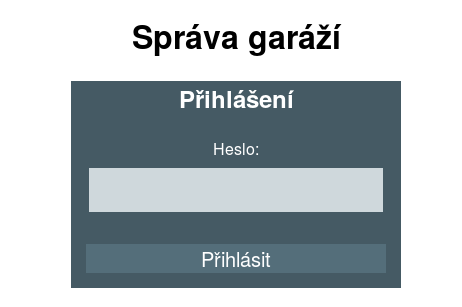
\includegraphics[width=0.5\textwidth]{images/login.png}
    \caption[Přihlašovací formulář webového rozhraní]{Přihlašovací formulář webového rozhraní.}
    \label{fig:login}
\end{figure}

\section{První přihlášení}

Pro první přihlášení je možné použít implicitní heslo \textit{password}. Poté je uživatel přesměrován na formulář se změnou hesla a vyzván ke změně z implicitní hodnoty (viz obrázek \ref{fig:password_change}).

\begin{figure}[h!]
    \centering
    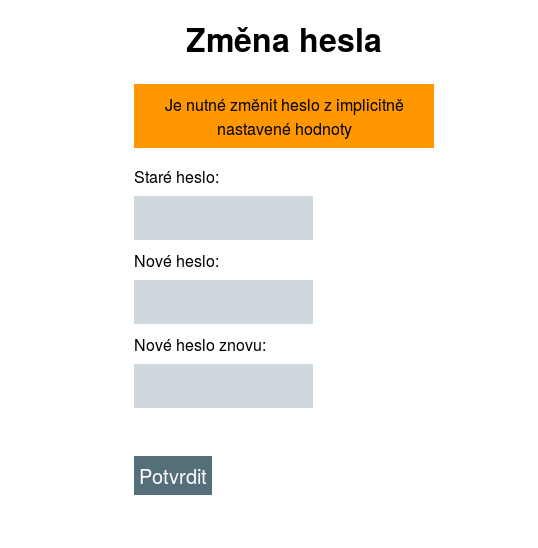
\includegraphics[width=0.5\textwidth]{images/pwd_change.png}
    \caption[Výzva ke změně hesla]{Výzva ke změně hesla.}
    \label{fig:password_change}
\end{figure}

\newpage

\section{Hlavní stránka}

\begin{figure}[h!]
    \centering
    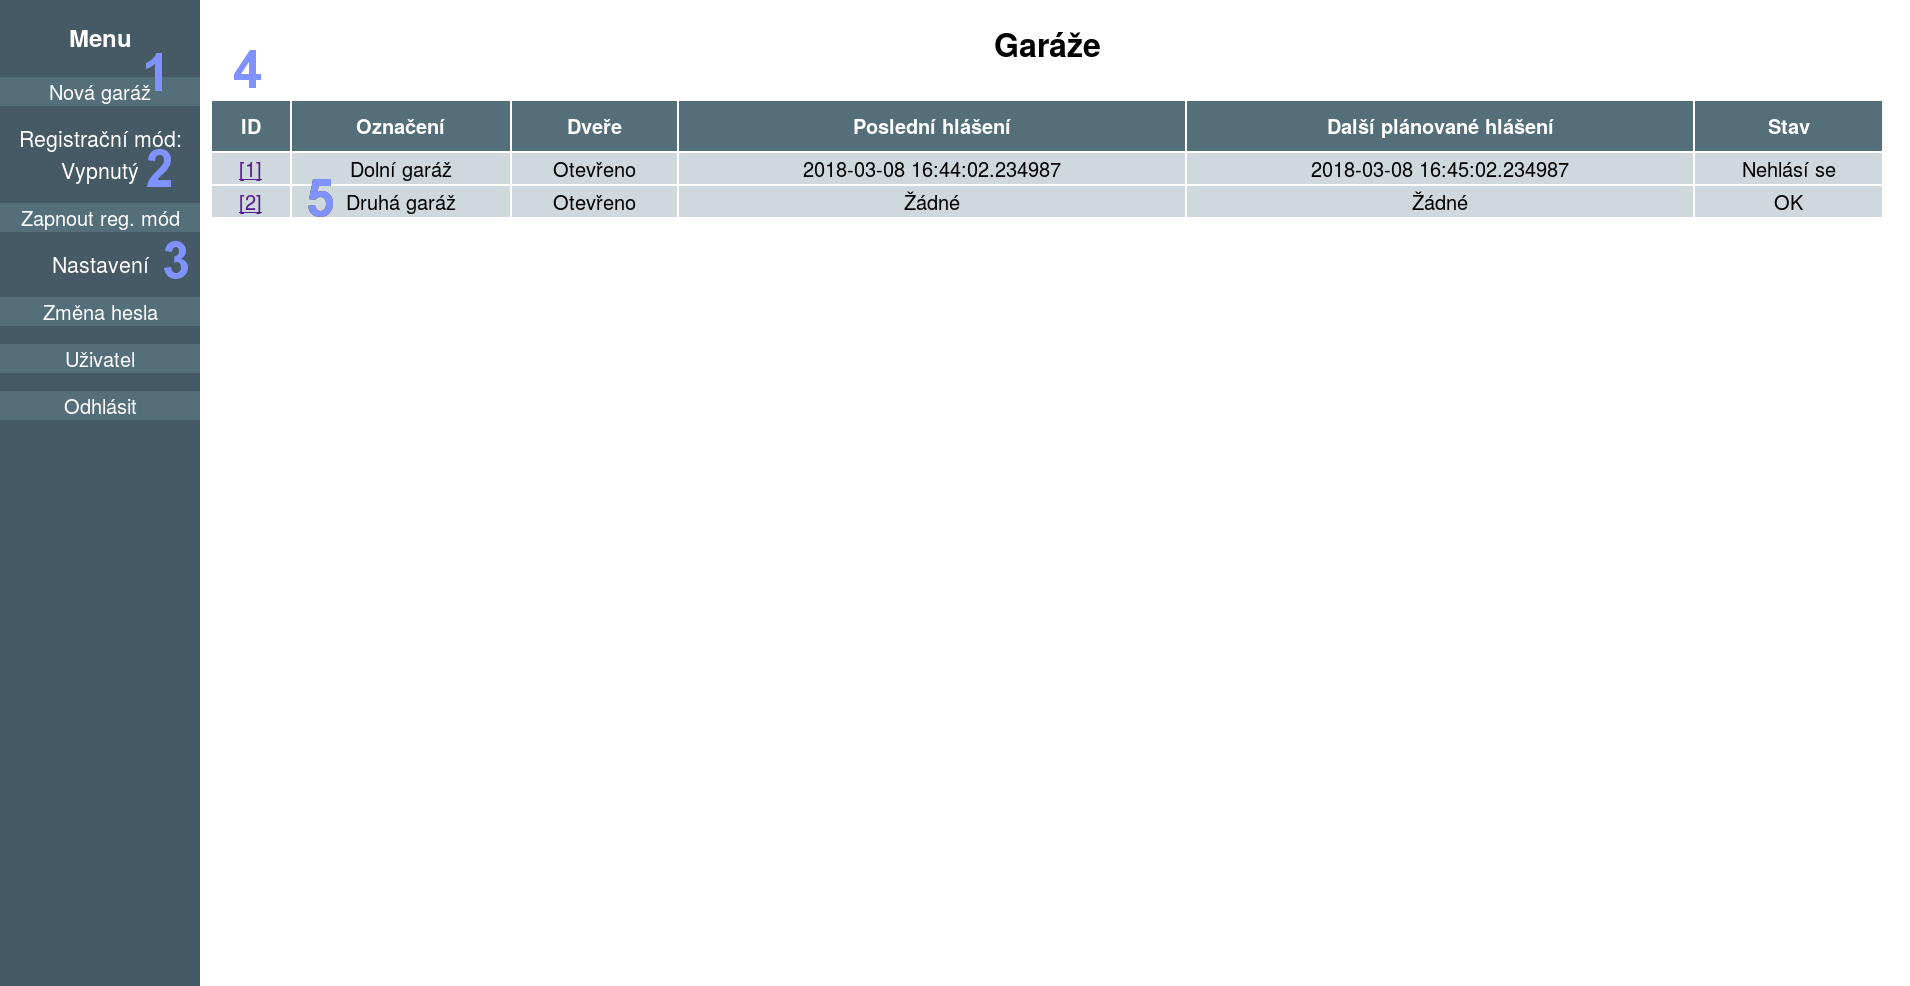
\includegraphics[width=\textwidth]{images/mainpage.png}
    \caption[Hlavní stránka aplikace]{Hlavní stránka aplikace.}
    \label{fig:mainpage}
\end{figure}

Po úspěšném přihlášení ze zobrazí hlavní stránka webového rozhraní. Zde má uživatel k dispozici následující možnosti (viz čísla na obrázku \ref{fig:mainpage}):

\begin{enumerate}
    \item \textbf{Nová garáž} -- vytvoření nové garáže pomocí uživatelského rozhraní. Nová garáž je přidána do seznamu garáží na této stránce.
    \item \textbf{Registrační mód} -- indikátor stavu registračního módu. Regstrační mód povoluje podřízeným systémům vytvářet nové garáže registračním požadavkem. Při registraci pomocí tohoto módu je podřízenému systému automaticky zaslán API klíč, a není nutné ho ručně nahrávat. Po zapnutní je registrační mód aktivní po dobu tří minut, poté se sám automaticky vypne.
    \item \textbf{Nastavení} -- uživatelské nastavení aplikace:
    \begin{itemize}
        \item \textbf{Změna hesla} -- možnost změny přístupového hesla do webového rozhraní.
        \item \textbf{Uživatel} -- viz sekci \ref{sec:guide_user_settings}.
        \item \textbf{Odhlásit} -- odhlášení z webového rozhraní.
    \end{itemize}
    \item Seznam sledovaných garáží (podřízených systémů):
    \begin{itemize}
        \item \textbf{ID} -- identifikátor garáže v systému, zároveň slouží jako odkaz na stránku garáže (viz sekci \ref{sec:guide_garage_page}).
        \item \textbf{Označení} -- Uživatelem zvolené označení garáže.
        \item \textbf{Dveře} -- Stav dveří garáže (otevřeno/zavřeno).
        \item \textbf{Poslední hlášení} -- Datum a čas posledního zaznamenaného hlášení.
        \item \textbf{Další plánované hlášení} -- Datum a čas dalšího plánovaného hlášení.
        \item \textbf{Stav} -- Stav garáže (OK, Nehlásí se, Detekce pohybu, Detekce kouře).
    \end{itemize}
    \item Záznam garáže.
\end{enumerate}

\newpage

\section{Stránka garáže}
\label{sec:guide_garage_page}

\begin{figure}[h!]
    \centering
    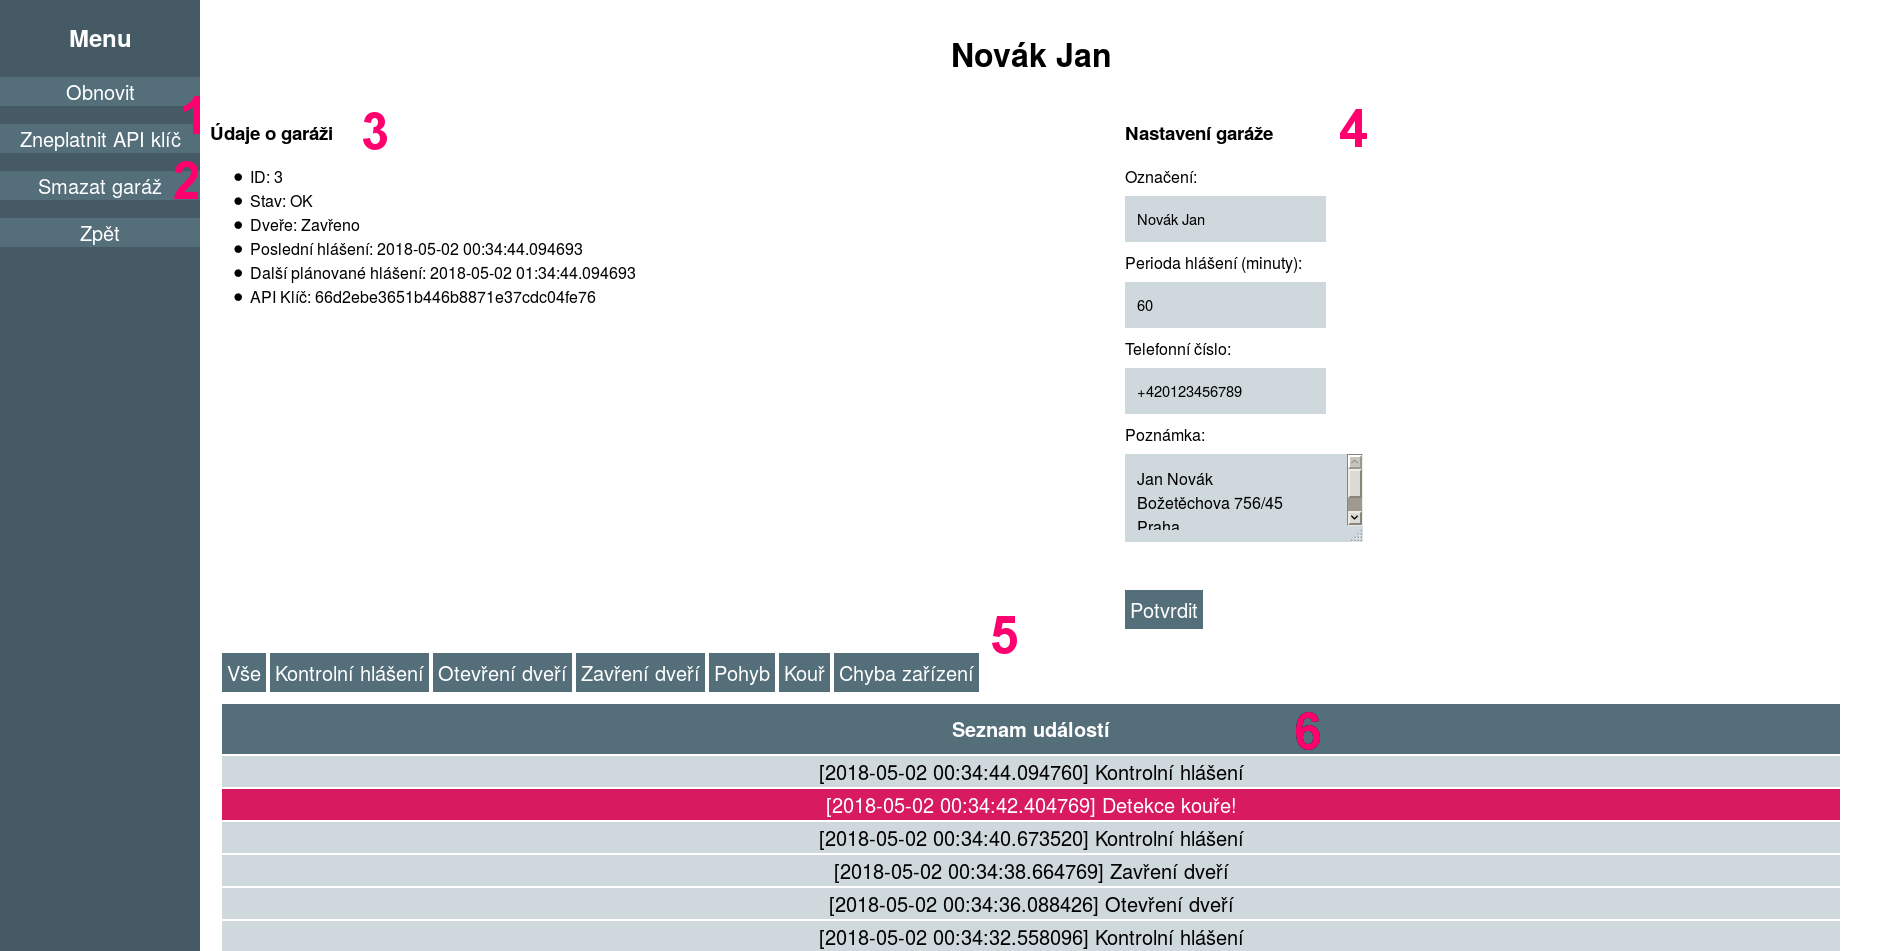
\includegraphics[width=\textwidth]{images/garage_page.png}
    \caption[Stránka garáže]{Stránka garáže.}
    \label{fig:garage_page}
\end{figure}

Na obrázku \ref{fig:garage_page} je zobrazena stránka konkrétní garáže. Zde jsou k dispozici tyto možnosti:

\begin{enumerate}
    \item \textbf{Zneplatnit API klíč} -- vygeneruje nový API klíč garáže. Po jeho vygenerování již nebude podřízený systém v této garáži moci zasílat nové události. Pro obnovení přistupu je nutné nahrát na systém nový klíč, případně vytvořit novou garaž pomocí registračního módu.
    \item \textbf{Smazat garáž} -- smaže zobrazenou garáž, včetně zaznamenaných událostí.
    \item \textbf{Údaje o garáži}, včetně API klíče.
    \item \textbf{Nastavení garáže}:
    \begin{itemize}
        \item \textbf{Označení} -- uživatelem zvolené označení, které se zobrazí na hlavní stránce.
        \item \textbf{Perioda hlášení} -- perioda kontrolních hlášení podřízeného systému (v minutách).
        \item \textbf{Telefonní číslo} -- telefonní číslo nájemce garáže. V~případě vyplnění budou upozornění týkající se garáže zasílána i nájemci. Telefonní číslo je třeba vyplnit včetně předvolby (+420 pro Českou republiku).
        \item \textbf{Poznámka} -- volitelná poznánka ke garáži (max 256 znaků).
    \end{itemize}
    \item \textbf{Filtry událostí} -- možnost filtrovat zobrazené události podle typu.
    \item \textbf{Události} -- tabulka zaznamenaných událostí, včetně data a času.
\end{enumerate}


\section{Uživatelské nastavení}
\label{sec:guide_user_settings}

V uživatelském nastavení může uživatel měnit e-mailovou adresu, na kterou nadřazený systém zasílá upozornění o změně stavu garáže. Může zde také tato upozornění úplně zakázat.